 %proofread!

%\documentclass[draft,jgrga]{agutex}
\documentclass[12pt]{article}
\usepackage{graphicx}
\usepackage{amsmath} %for help with the bracketed conditional equations
\usepackage{multirow}
\usepackage{caption}
\usepackage{array}
\usepackage{natbib}
\usepackage{xcolor}
\usepackage{float} %for figure purposes
\usepackage[affil-it]{authblk} %to get the affiliations
\setlength{\abovecaptionskip}{5pt plus 1pt minus 1pt}
%todonotes can't be run on this login on melt because apparently pfg/tikz are old or something
%\usepackage[disable,colorinlistoftodos, textwidth=65mm, shadow]{todonotes}
%\usepackage{authblk}

\usepackage{tabularx}
%\usepackage{lineno}
%\linenumbers*[1]

%\noindent $>$latex file \\
%\noindent $>$dvips -P pdf -o file.ps file.dvi \\
%\noindent $>$ps2pdf13 file.ps file.pdf

%\authorrunninghead{Gail Gutowski	Portfolio in Applied Statistical Modeling}
%\titlerunninghead{Gail Gutowski	Portfolio in Applied Statistical Modeling}

\date{}
\renewcommand{\abstractname}{Executive Summary}

\begin{document}

\title{Age-depth relationship and associated uncertainty of englacial radar layers in Marie Byrd Land, West Antarctica\bigskip\bigskip}

\author{\textbf{Gail Gutowski}, Charles Jackson, Duncan Young, Donald Blankenship}
\affil{Institute for Geophysics, University of Texas at Austin}

\date{\parbox{\linewidth}{\centering%
  \endgraf\bigskip\bigskip\bigskip
  Completed for Portfolio in Applied Statistical Modeling \endgraf}\bigskip\bigskip\bigskip}
  


%\maketitle
%\thispagestyle{empty}
%
%\begin{center}
%  \noindent\begin{tabular}{ll}
%\makebox[3in]{\hrulefill} \\
%Dr. Charles Jackson, Research Advisor \\[10ex]% adds space between the two sets of signatures
%\makebox[3in]{\hrulefill} \\
%Dr. Matthew Hersh, Faculty Advisor \\
%\end{tabular}
%\end{center}


\pagebreak
\pagenumbering{roman}
\begin{abstract}
%We present a new depth chronology for ice near Byrd ice core which accounts for uncertainties in ice penetrating radar and ice core dating. Our chronology consists of an ensemble of age-depth profiles representing the physical range of uncertainty associated with prominent radar reflectors in the ice. These profiles are useful for inferring ice strain rates and ice velocities, which are necessary for modeling ice dynamics.

%We present estimates of the age-depth relationship for ten radar reflectors in the Marie Byrd Land sector of West Antarctica, near the WAIS Divide and Byrd ice core sites. We compute a range of ages for these radar reflectors which incorporate uncertainties from radar and ice core measurements. An ice flow model is used to simulate the depth dependence of layers. The Metropolis-Hastings algorithm is used to invert for ice flow parameters which lead to age-depth profiles consistent with observations to within uncertainty. 

%We present ten layers that have been traced and dated in this region to a depth of 1400 m. We find age-depth uncertainty introduced by radar is approximately 2 m and is constant with depth below 168 m. Combined with an assumed 3\% uncertainty in age in the ice column from ice core dating, we find that some pairs of spatially distinct radar horizons are consistent with being isochronous deposition events. This information is useful in determining the duration of past events affecting ice fabric, such as volcanic eruptions, which deposit dust with a prominent dielectric contrast in the ice column. Ambiguities in the age-depth relationship also suggests the importance of including a complete accounting of uncertainty, including chronologic uncertainty, to fully describe the dynamic evolution of the ice sheet. 

\smallskip
The West Antarctic Ice Sheet (WAIS) is thinning and has the potential to contribute substantially to sea level rise in the future. Current understanding of ice sheet feedbacks which may compound or regulate glacial melting of the WAIS is limited. To better predict future response of the WAIS to climate change, we propose exploring the past behavior of the ice sheet to time-varying climate. 

We investigate the evolution history of the WAIS since the Last Glacial Maximum by combining observations from ice-penetrating radar and deep ice cores to determine the age-depth relationship of WAIS ice. Simple ice flow models are used at each ice core site to determine physically consistent flow parameters which preserve the dependence of layer depth and age within the ice column.

Direct measurements of ice age as a function of ice sheet depth are determined visually, chemically, and electrically for the WAIS Divide and Byrd ice cores in central West Antarctica. Coincident with the ice core sites are ice-penetrating radar surveys which extend for hundreds of kilometers and consist of ice sheet cross sectional data. The cross sections contains bright, continuous radar reflection horizons which we assume to be related to isochronous ice accumulation layers. These englacial layers can be extensively tracked from the ice core sites throughout central West Antarctica.

We seek to assign ages to these trackable radar layers by relating them to the ice core chronologies via an ice flow model. To do so, we sample both radar depth and ice core age uncertainty. We include three sources of error for the radar-derived layer depths. Age uncertainty is incorporated via Bayesian inversion of ice flow parameters which acknowledges errors in the ice core chronology.

The result samples the posterior age-depth profile near the ice core site and can be directly mapped to radar-detected layers extending throughout the West Antarctic Ice Sheet. The age-depth profile computed using this method makes good use of observations in the area while accounting for uncertainties in both observations and existing understanding of ice flow physics.

%paragraph comparing results between the two cores
\end{abstract}

\pagebreak

\tableofcontents

\pagebreak

\section{Introduction}
\pagenumbering{arabic}
%Outline of new intro:
%Why -- predict future ice sheet response
%how -- englacial layers
%	-- window into ice sheet
%	-- possible with remote sensing
%	-- records/preserves ice sheet history
%	-- spatially extensive
%	-- correlated to ice cores = dates
%but/how -- need to incorporate uncertainty, which 	can come from several sides
%what -- probabilistic distribution of ice age throughout thw catchment, MBL (see proposal language)

Ice sheet response to changes in climatic conditions in the past can be useful for anticipating the response of the West Antarctic Ice Sheet (WAIS) to current global warming. Understanding the past dynamics of the WAIS during similar climates could inform estimates of modern WAIS stability and predictions of future WAIS melt with the potential to contribute to sea level rise.

Age-depth profiles are one tool to explore ice dynamics and accumulation history by exploring the distribution of ice age as a function of depth. In recent years, ice-penetrating radar has made it possible to extend one-dimensional age-depth profiles measured at ice cores over hundreds of kilometers in the West Antarctic Ice Sheet \citep[e.g.][]{neumann2008,holt2006}. This allows for englacial layer dating over an extensive three-dimensional region of the ice sheet. Layer geometry can then be used to investigate WAIS flow during past climate regimes. Deformation in the shape of these layers, generally deposited in flat sheets at the surface, may be indicative of ice flow history \citep[e.g.][]{siegert2004}.

Errors arise in both radar-derived layer depths and ice core age profiles. Such errors become larger at greater depths, where strain thinning and complex past flow hampers interpretation of the ice core chronology and layer identification. It is necessary to account for these sources of uncertainty when mapping dates to englacial radar layers. Several sources of error related to ice composition and radar system specifications are considered. To quantify the age uncertainty, we use a Bayesian method to invert for a distribution of physically-motivated ice flow model parameters capable of reproducing the observed ice core chronology to within uncertainty. Use of simple flow models preserves the physical dependence of relative layer ages in the ice column. 

The resulting ensemble of age-depth profiles sample the posterior distribution of age-depth at the ice core sites. This information can then be propagated to most of the central WAIS via layer tracking using seismic imaging software, potentially revealing a vast amount of information about layer geometry and paleo ice flow.
%It is important to understand uncertainty in ice-penetrating radar data and how that uncertainty may affect interpretation of paleo ice evolution. The accuracy of dating englacial radar horizons depends on uncertainty in radar observations and in ice-core dating. \cite{eisen2004} evaluated this uncertainty for ground-based radar in the top 100 m of the East Antarctic Ice Sheet. We approach the problem using ice-penetrating radar observations of the West Antarctic Ice Sheet (WAIS) near the WAIS Divide and Byrd ice cores and consider radar horizons in the upper 1300 m of the ice column. 

%We use an ice-core-derived chronology and a one-dimensional ice flow model to evaluate age and depth uncertainty of the ice using a Bayesian framework. We present the resulting ensemble of age-depth profiles, which represents a probabilistic estimate of the relationship between age and depth. We then propagate the profile through continuous ice-penetrating radar horizons throughout Marie Byrd Land. The result is a three-dimensional map of layer age and depth in a large region of the WAIS. Such information can be used to test hypotheses about past ice dynamics and boundary conditions, including surface mass balance.

\section{Data}

\subsection{Radar Data}
%*See Marie's paper for language*
Several surveys have acquired ice-penetrating radar-echo sounding (RES) data of the WAIS, including Airborne Geophysical Survey of the Amundsen Sea Embayment \citep[AGASEA,][]{holt2006}, Geophysical Investigations of Marie Byrd Land Evolution (GIMBLE), and others \citep[e.g.][]{bedmap2}. The data includes two-way travel times (TWTT; the time it takes for a radar pulse to be transmitted, reflect off an englacial layer, and return to the receiver) in microseconds collected using a 60 MHz center frequency. GIMBLE data was collected with the High Capacity Airborne Radar Sounder (HiCARS) system. HiCARS uses a 1 $\mu$s chirp width with a 15 MHz bandwidth corresponding to a 100 ns pulse width after compression (8.4 m in ice) and a 6.4 kHz pulse repetition frequency (PRF). Signals were digitized at 20 ns intervals and coherently stacked ten times, log detected and incoherently stacked five times to yield records every 22 m along-track (Young and others, 2011). HiCARS data was used to determine the age-depth profiles at both the WAIS Divide and Byrd ice core sites. %%%%%%%%\textcolor{red}{Data collected prior to 2008 (AGASEA, Byrd Subglacial Basin surveys) pre-dated HiCARS and instead used the UT/TUD (University of Texas/Technical University of Denmark) radar system. The UT/TUD system was acquired with a pulse width of 290 ns (~24.4 m in ice) and a PRF of 12.5 kHz. Log-detected signals were digitized at 16 ns intervals for 65.5 sec and incoherently stacked 2048 times to generate a trace every ?20 m along-track \citep{Carter2009}.} 

We also use ice-penetrating radar collected by the CReSIS Multi-Channel Coherent Radar Depth Sounder \citep[MCoRDS;][]{bedmap2} to extend the age-depth information throughout the WAIS domain. The MCoRDS system operates in a frequency range between 180 MHz and 210 MHz. It uses multiple receivers and an adjustable bandwidth up to 30 MHz. This leads to 4.5 m vertical resolution in ice and 30 m along-track sampling \citep{Leuschen2000}.

Ten radar layers were traced through radargrams from these surveys based on peaks and troughs in processed signal amplitude. Tracing was completed using the seismic imaging softwares \textit{GeoFrame} and \textit{LandMark's} Decision Space Desktop. These softwares employ semi-automated tracking algorithms to follow peaks in return signal using an adjustable travel-time window. The ten layers were selected for their prominent signal and continuity through the Marie Byrd Land (MBL) domain in central West Antarctica. Layer traceability may diminish along a single RES flight line due to discontinuities or waning signal, but crossovers between RES flight lines allow for extensive layer tracking. The ten layers included in this analysis are shown in Figure~\ref{fig:radargram} in a radargram of an ice sheet cross section near the Byrd ice core.

%Englacial layers observed by ice-penetrating radar are a result of temporally varying properties of deposited snow. The physical properties of snow accumulating on the ice sheet surface contains information about climatic conditions at the time of deposition. For instance, the oxygen isotope, $\delta^{18}O$, can be used as a proxy for temperature. Over time, the surface layer is covered with accumulation of subsequent years and becomes buried in the ice column. Differences in chemical composition of the ice lead to variations in electrical conductivity observed by the radar as distinct layers. 


\subsection{WAIS Divide ice core chronology}
The WAIS Divide ice core (see Figure~\ref{fig:radarmap}; 79.48$^{\circ}$S, 112.11$^{\circ}$W), is the most recently drilled deep ice core to be drilled in Antarctica \citep{buizert2015}. Annual layer counting to 2850 m depth and methane synchronization to 3404 m depth were used to determine an age-depth chronology for the ice core. The core reached 50 m above the estimated bed depth to avoid contaminating the basal hydrology system. The oldest ice in the core has been dated to $\sim$68ka at high resolution (0.5 m to 2m at depth). High resolution and precision are achievable at the WAIS Divide site because of the locally high accumulation rate at the divide and the precision of the methane synchronization method used to determine the deep chronology.


\subsection{Byrd ice core chronology}

The Byrd ice core (see Figure~\ref{fig:radarmap}; 80.0167$^\circ$S, 119.5167$^\circ$W), drilled in 1968, was the first in Antarctica to extend to bedrock \citep{gow1968}. Damage to the ice core above 88 m prohibited the traditional approach of annual layer counting in the shallow portion of the core. However, a shallow core drilled nearby in 1989 (NBY89) enabled \citet{langway1994} to complete a chronology for the top 164 m of the ice column. Below 88 m, the electrical conductivity method (ECM) was used to date the ice core \citep{hammer1994}. The ECM method measures variations in electrical conductivity. Between 300 m and 900 m, brittle ice precluded sufficient ECM measurements, so \citet{hammer1994} instead fit the chronology with three piecewise linear functions. The resulting layer-thickness profile was integrated from surface to depth to obtain an age-depth relationship for the length of the ice core.

\citet{hammer1997} present a volcanic chronology of the Byrd ice core based on this previously-derived timescale in which volcanic events were matched to peaks in electrical conductivity, consistent with the presence of ash in the ice column. The chronology includes dated volcanic events between 709 BP and more than 18,000 BP, corresponding to depths ranging from 97.8 m to 1890 m below the 1968 surface of the Byrd ice core. We use part of this volcanic record to 1358 m depth (corresponding to 20,594 a) as an observational constraint on our age-depth profile.



\section{Sources of Uncertainty}\label{unc}
%There are many sources of uncertainty inherent to the way in which data is collected, analyzed, and understood. We have included the following sources of uncertainty in our analysis.

\subsection{Radar Depth Estimates and Uncertainty }\label{radunc}
%See Marie's paper for language
First-order layer depth beneath the ice surface is derived from radar-acquired TWTT using constant electromagnetic (EM) velocities in ice and air. These velocities are derived using a dielectric constant in ice of $\epsilon$$^{'}$ = 3.17 \citep{peters2005,gudmandsen1971} and the common relation $C_{ice} = C_{air}/\sqrt{\epsilon^{'}}$. Mean EM signal velocity in ice and air are used to determine first-order depth and are presumed constant (300 m/${\mu}$s and 168.75 m/${\mu}$s, respectively), though errors may exist in EM velocity in ice, as described below.  

We consider three sources of error in radar-derived layer depths: 1) variations in the EM signal velocity in ice due to ice temperature and fabric, 2) vertical resolution limitations resulting from digitized pulse width sampling effects, and 3) measurement errors in the density profile used to determine the firn depth correction.

EM velocity in ice varies from 168 to 169.5 $m/{\mu}s$ \citep{fujita2000}, leading to increasing uncertainty with depth. Variations in this velocity result from ice temperature, crystal structure, isotropy, and other ice fabric effects. Because of the complexity of local ice properties which may affect the velocity at any location and depth, we make the simplifying assumption that this error is uniform. For each iteration of the method, we sample from the uniform distribution \textit{v} $\sim$ U(168 $m/{\mu}s$, 169.5 $m/{\mu}s$) to select the velocity for which the depth will be determined. 

Again assuming these errors are normal, we independently randomly sample each error from a normal distribution with mean 0 and standard deviation equivalent to the quoted depth error above. 

Vertical resolution varies based on each radar system's measured radar pulse width \citep{millar1982}. The finite pulse width means that an infinitesimally thin layer of ice will appear in the survey to have a finite width. The error in phase sampling of this pulse is taken to be $\frac{\lambda}{4}$%for data with high signal-to-noise ($\lambda$ is the wavelength of the electromagnetic pulse)
. The sampling rate for the data used here varies from 5 ns to 20 ns. Conservatively, we assume a 10 ns resolution when tracking the phase of layer detections. We then randomly sample from a normal distribution with mean 0 and standard deviation %%%\textcolor{red}{X m} 
(10 ns) for the HiCARS radar system, which was used to determine the age-depth profile at each ice core.  

All layers of interest in this analysis are deeper than the firn layer in both ice cores. A firn depth correction is therefore added to the depths of all radar layers in the ice column to accommodate the underestimation of depth if the firn layer is neglected. The firn correction is computed using the usual \citet{dowdeswell2004} relation:

\begin{equation}
z_f = \frac{K}{n^{'}_{i}}\int{(\rho_{i} - \rho(z)) dz}
\end{equation}
where K is 0.85 m$^{3}$Mg$^{-1}$ \citep{Robin1969}, $n^{'}_{i}$ is the refractive index of ice (=1.78), $\rho_{i}$ is the density of ice (=0.917 Mg m$^{-3}$) and $\rho(z)$ is the density of ice at depth \textit{z} with units Mg m$^-3$.

Ice density data as a function of depth were obtained from the original analysis of the ice core \citep{gow1968} and from a shallow core near the main WAIS Divide core \citep{kreutz2011}. The data were used to account for the varying density of ice and subsequent variations in electromagnetic wave speed through the firn layer at the top of the ice sheet.  The WAIS Divide Ice core includes a comprehensive density error analysis as a function of depth. To incorporate the density error, we assume the errors are gaussian and sample from the density distribution as a function of depth. A firn correction is computed for each sampled firn layer and the resulting firn depth distribution, also normal, is used to characterize the firn depth error. 

%%%%%%%%%%%(\textcolor{red}{how much is firn correction (distrib) at each ice core site})

It is important to note that the computed depth of each layer is relative to the ice surface as also measured by the HiCARS radar. While each layer may have errors independent of the others, errors in the distance of the surface from the acquisition aircraft are systematic across all observed layers. Therefore, a randomly sampled error due to the vertical resolution is computed for the surface and the same error is applied to all radar layers. Additionally, all layers of interest lie below the computed firn layer at each ice core site. The firn correction error is therefore also systematically applied to all subsequent radar layers. 

To compute the total uncertainty in depth to each layer, we sample each of the three errors described above to construct a depth distribution characteristic of the overall uncertainty. This distribution is comprised of sampling each error 10,000 times. While firn and velocity errors are the same for all layers in a single ice column, the pulse width error is sampled for each layer independently. For the \textit{ith} radar layer in the column:

\begin{equation}\label{deptheqn}
Depth_i = \frac{TWTT}{2}*\overline{v} + \epsilon_{v} + \epsilon_{PW} + \epsilon_{firn}
\end{equation}
The results show overall depth uncertainty increases with depth, as expected. 

%%%%%\textcolor{red}{what are the values? make a fig of depth v. unc}

\subsection{Age Estimates and Uncertainty}\label{ageunc}

We interpret the englacial layers as isochronous under the assumption that each continuous layer of ice which shares dielectric properties was deposited on the surface at same time \citep{eisen2004}. Estimates of the age of ice throughout each ice core is completed using visual layer counting, isotopic analysis such as methane synchronization \citep{buizert2015}, or the electrical conductivity method \citep{hammer1997}. Absolute dates are obtained by correlating the Antarctic ice cores with absolute records from the Greenland Ice Sheet such as the GRIP %%%%%%%\textcolor{red}{What does GRIP stand for and citation} 
ice core. Absolute dating is also possible using correlation with known and dated global volcanic events and northern hemisphere ice cores. 

Estimates of errors in dating the WAIS Divide ice core are approximate and according to expert opinion. We expect larger age errors in ice deeper in the ice sheet, where shear thinning results in layers that are more difficult to distinguish from one another and where disruptions in shallower parts of the ice core can contribute error to dating deeper layers. We assume errors are 3\% of the ice age, which is conservative for modern ice cores (such as WAIS Divide) according to expert opinion (personal communication T.J. Fudge, 2013). Without additional information for uncertainty analysis, we contend this is an appropriate first-order description of the age errors. %%%%%\textcolor{red}{more about what makes this uncertain}

The Byrd ice core chronology is uncertain due to damage in the upper part of the core, a zone of brittle ice between 788 m and 900 m depth, subjectivity in the interpretation of ECM results, among other reasons. \citet{hammer1994} suggest a precision of $\pm$ 1000 years for 20 ka ice due to subjectivity in the ECM technique. They also give an approximate accuracy of 1 ka ice as $\pm$ 500 years. The volcanic chronology developed by \citet{hammer1997} quotes $\pm$ 500 years for the prominent Old Faithful radar horizon observed to be approximately 17,400 a old. Due to a lack of uncertainty analysis of the ice core chronology, we assume an uncertainty distribution that is 3\% of the observed age of the ice column, the same assumed for the WAIS Divide ice core. For example, this assumes that Old Faithful is of age 17,400 $\pm$ 522 a and that a layer of age 10 ka has uncertainty $\pm$ 300 years. 

%Each year, fresh snow accumulates on top of the ice sheet, burying the previous season's snowfall. As layers of ice are advected into the ice sheet, they become thinner as the ice is compacted due to increasing overlying ice and shear thinning from ice flow. This thinning makes it increasingly difficult to distinguish one between horizons at depth. In shallow regions, it is possible to count layers by eye to determine the age of near-surface isochrones; however, this is harder to do deep in the ice sheet. The uncertainty associated with determining ages for ice layers is therefore a function of depth. 

%The upper part of the original 1968 Byrd ice core was too damaged to count annual layers. However, in 1989, a shallow core dubbed NBY89 was drilled nearby which enabled \citep{langway1994} to complete a chronology for the top 164 m of the core. Using the ECM method \footnote{ The Electrical Conductivity Method (ECM) is another approach to dating ice. It involves measuring the conductivity of ice at different depths \citep{hammer1994}. This conductivity is associated with the composition of the ice, characterized by its acidity level. Layers of ash embedded in the ice, for example, will have a distinct conductivity. The ECM method is particularly useful in deep parts of the ice column where it is difficult to otherwise distinguish isochronous layers due to layer thinning.}, they matched 3 volcanic events to the original ice core with an uncertainty of $\sigma_{age} = \pm$ 2 yr for the upper 1360 a of the ice core.

%Isotopic dating is common among ice core chronologies. Landmark events for concentrations of Beryllium-10, methane, and fluorine (to name a few) are matched to chemical analyses of the ice \citep{schwander2001} at different points in time. Accepted dates for these events are then mapped onto the ice core. 

%We adopt the following estimates of uncertainty to accompany the isotopic dating, though no comprehensive review of uncertainty from these methods is available. The end of the Younger Dryas period is correlated between the GRIP and Byrd ice cores using CH$_4$. This method indicates an uncertainty of roughly $\sigma_{age} = \pm$ 150 yr for the period between 1360 a and 11.5 ka \citep{ blunier1998, schwander2001}. This incorporates uncertainty in the $\delta$age estimate on the GRIP and Byrd cores ($\pm$ 100 yr) as well as the CH$_4$ match between the GRIP/Byrd ($\pm$ 100 yr). For the period between 11500 a and 17320, we adopt an uncertainty of $\sigma_{age} = \pm$ 300 yr \citep{schwander2001}. This value is the result of stratigraphic layer counting near a prominent fluoride peak at Byrd station, tuned by matching CH$_4$ during the Younger Dryas period.

%For layers older than 17320 a, we assume $\sigma_{age}$ = 2 ka based on U/Th dating of the Laschamp geomagnetic excursion \citep{schramm2000}. Note that we include this uncertainty for completeness; the ten radar horizons of interest in this analysis are believed to be younger than 17320 a.

%Table~\ref{age_unc} summarizes the uncertainty we assign to observed ages as a function of depth.


\section{Method}\label{method}
The depth-age profile will be determined at both the WAIS Divide and Byrd ice cores for comparison and to potentially reduce uncertainties at the Byrd ice core. The ten layers selected for this study are observed near both ice cores and can be directly tracked continuously between the two. As a result, the age of each layer determined at the two ice cores sites should be consistent to within uncertainty.

Ice flow models are used to determine the age-depth profile in the ice sheet because of the dependence of the age of layers in the ice column on each other. We use the ice flow model to enforce the constraint that older ice is deeper in the ice sheet than younger ice. Use of the ice flow model also preserves the integrative effects of changes in accumulation rate and variations in strain rate with depth. Different ice flow models were used for the WAIS Divide and Byrd ice cores because of differences in their position on the ice sheet. The ice flow physics at an ice sheet divide are more straightforward because the velocity of ice is primarily vertical. Ice flow off the divide, such as near the Byrd ice core, can be more complex. The two ice flow models are described below.

\subsection{WAIS Divide ice core flow model}
Flow at the WAIS Divide ice core can be simply explained by the Dansgaard-Johnsen (D-J) model \citep{dansgaardjohnsen1969}. We implement the version of this model described in \citet{schwander2001}, with parameters \textit{r}, the ratio of horizontal ice velocity at the bed to that at the surface, and \textit{q}, the accumulation rate, shown in Equation \ref{divideflow}. %The parameter \textit{r} is considered a metric of strain rate.

\begin{equation}\label{divideflow}
age(z) = \int_{z}^{H} \frac{dz'}{\epsilon_z' q(z')}
\end{equation}
where
\begin{center}
$    \epsilon_z=
    \begin{cases}
                 1-k(H-z), & h \leq z \leq H \\
                  kz(r+\frac{1-r}{2h}z), & 0 < z < h
    \end{cases}
$
and
$
k = \frac{2}{2H - h(1-q)}
$
\end{center}
\textit{H} is ice thickness in ice equivalent, \textit{z} is height above the bed, and \textit{h} is the D-J transition depth fraction where the strain rate profile breaks from the Nye model result and decreases linearly to zero at the base of the ice sheet. This transition depth, \textit{h}, is assumed to be 0.7 at the WAIS Divide ice core site. Future work will allow this to vary as a free parameter, with prior U $\sim$(0.5, 0.8).

Priors on \textit{r} and \textit{q} are applied to specify conservative ranges of physically realistic values on the uncertain parameters. 

\begin{center}
q $\sim$ U(0, 0.3) \\
r $\sim$ U (0, 1)
\end{center}
Uniform priors are used for both parameters because no reliable distribution information is known beyond reasonable minimum and maximum values. For accumulation rate, \textit{q}, we conservatively assume WAIS accumulation is between 0 and 30 cm/year during the period of ice deposition.  We allow \textit{r} to take any value between 0 and 1, which assumes the basal ice motion is always equal to or less than the ice surface velocity. 

Several approaches to selecting accumulation parameter values will be explored. The current analysis determines a constant value of accumulation for the entire ice column, which is not realistic in the presence of changing climate over time. Variable accumulation rate over time is a more likely scenario, but it is expected there is some interannual dependence of accumulation rate which must be preserved. To accomplish this, future work will compare this analysis to that conducted with two other methods of determining accumulation rate. 

The first will invert for time-varying accumulation rate as a fraction of present accumulation rate according to a theoretical temperature-related function described in \citet{morse2002}. Applying a climate-related functional form of accumulation rate, though uncertain, maintains the integrity of the dependence of accumulation rate on climatic conditions. The other method will determine accumulation rate values in a stepwise manner in the same depth regimes as described in Section~\ref{byrdflow} for the Byrd ice core flow model. These regimes are based on transitions in layer thickness measured at the Byrd ice core site. They will be approximately correlated to WAIS Divide depths using the relative depth of englacial layers tracked between the two ice cores. This approach to estimating accumulation rate history benefits from its basis on measured observations at the Byrd ice core, though using layer thickness as a proxy for accumulation rate is a simplifying assumption.

\subsection{Byrd ice core flow model}\label{byrdflow}
At the Byrd ice core site, we use an ice flow model derived for conditions at the Byrd ice core by \citet{morland2009} to determine the age of internal layers near the Byrd ice core drilling site in Antarctica. Flow assumptions from the previous section must be relaxed to accommodate the off-divide Byrd ice core, specifically consideration of non-vertical strain rate components. The \citet{morland2009} model has the form:
\begin{equation}
\begin{array}{l}
\displaystyle \frac{\overline{z}}{h_0} = \frac{1}{1 - r} [1 - exp(-s \overline{t})]\\
\\
\displaystyle \overline{z} = h_0 - z\\
\\
\displaystyle r = \frac{b}{q}\\
\\
\displaystyle s = s_ds_0\\
\end{array}
\end{equation}
where depth, $\overline{z}$, is defined to be 0 at the base, $h_0 =$ 2164 m is the depth at the ice sheet surface, \textit{b} is basal melting rate, \textit{q} is the accumulation rate, and $\overline{t}$ is the age corresponding to $\overline{z}$. The optimum constant strain rate, $\textit{s}$, is used to achieve reasonable correlations between the model and observations; $s_0$ is the initial strain rate and $s_d$ is determined empirically for the Byrd ice core to be $s_d$ = 0.722 for the Byrd ice core \citep{morland2009}. The model assumes isostatic equilibrium, constant ice density, uniform strain rate in $\textit{z}$, and $\textit{r}$ $<$ 1 (i.e. nonnegative mass balance in the ice column). Further, while depth in the model, $\overline{z}$, is defined so that $\overline{z}$(base) $=$ 0, the following analysis is discussed in terms of depth $\textit{z}$, where $\textit{z(surface)} = 0$.

Note that it is difficult to know accumulation rate on its own due to layer thinning at depth within the ice column. As such, we consider layer thickness instead of layer accumulation because it can be physically measured using the techniques described previously. We use a stepwise function to parameterize accumulation in four depth regimes:

$$
z = \left\{ \begin{array}{rl}
z_1 & \mbox{  z $< 150$ m } \\
z_2 & \mbox{  150 m $\le$ z $< 1024$ m} \\
z_3 & \mbox{  1024 m $\le$ z $ < 1294$ m} \\
z_4 & \mbox{  z $\ge$ 1292 m }\end{array} \right.
\\
$$
These regimes were chosen based on a linear piecewise function of layer thickness developed by \citet{hammer1994} in which slope changes are observed at the above transition points. We use the flow model to invert for accumulation as a function of depth, $\textit{q}$, and strain scale factor, $\textit{s}$, \citep[][see]{morland2009} using an observed age-depth relationship. 

%We use the resulting parameters to evaluate the age of the ten radar layers of interest. The inversion is done using a Markov Chain Monte Carlo technique known as the Metropolis-Hastings algorithm \cite{metropolis1953}. %%%%%%\textcolor{red}{what are the prior values?}

% For this analysis, we use the calculated strain rate to express accumulation from the model in terms of layer thickness for comparison to observations according to the simple strain thinning relationship:

%\begin{equation}
%\.{b} = s \lambda
%\end{equation}
%\\
%where $\.{b}$ is accumulation and $\lamdba$ is layer thickness which are related by the (assumed uniform) vertical strain rate.

\subsection{Bayesian inversion of ice flow}\label{metrop}
We are interested in finding appropriate flow model parameters which lead to age-depth profiles consistent with the observed ice core timescales. To do so, the flow models are inverted for the parameters described above. Acceptable parameter values are those which describe flow consistent with the observed age-depth relationship at the ice core sites. 

We implement a Random Walk Metropolis algorithm (described here) to use prior knowledge about the model parameters to develop a joint posterior distribution of the parameters. We use truncated uniform priors on all parameters, allowing them to take on values within a physically reasonable range, as described in the preceding sections.  The model is initialized using random parameter values within these ranges.

At each model step, we evaluate the age determined by the flow model at every depth in the ice column (up to 3404 m for the WAIS Divide ice core and 2164 m for the Byrd ice core) based on proposed sets of parameters.  An associated likelihood is evaluated as a measure of the model-data misfit for each proposal. The log likelihood is described in equation~\ref{cost}:

\begin{equation}\label{cost}
cost = log(likelihood) = \frac{(Age_{model}~ - ~Age_{obs})^2}{(2\sigma_{obs})^2}
\end{equation}
where $Age_{model}$ comes from evaluating the ice flow model for an ice core site given proposed parameters. $Age_{obs}$ and $\sigma_{obs}$ come from the WAIS Divide ice core chronology and the volcanic age-depth function for the Byrd ice core, respectively. We allow for the uncertainty in $Age_{obs}$ ($\sigma_{obs}$) to loosen the constraint on how closely the $Age_{model}$ must match $Age_{obs}$ to be acceptable. 

At each iteration, the algorithm makes a decision about whether or not to accept the combination of parameters based on the cost function. If the cost of the \textit{n}th iteration is less than the cost of the \textit{(n-1)}th iteration, the set of parameters is accepted. This means that the \textit{n}th set of parameters is a better fit to the data, indicated by a decreased cost. If the cost has not decreased, there is still a chance the algorithm will accept the parameter set. If the cost of the \textit{n}th iteration is greater than the cost of the \textit{(n-1)}th iteration, the set of parameters is accepted with probability $exp[-\frac{cost_n~-~cost_{n-1}}{2}]$. This enables a full exploration of parameter space in the event there are multiple equally acceptable solutions. Due to the uncertainty in the observed ice core chronology and flow model parameters, we expect this to be the case. After determining the suitability of the parameters and either saving or discarding them, the algorithm continues to iterate, randomly walking through parameter space for 10,000 iterations. 

The resulting ensemble of flow model parameter sets describe 10,000 flow models suitable to describe the local physics at the two ice core sites to within uncertainty. We sample from this distribution to characterize the age uncertainty when determining the age of each observed radar layer.

\subsection{Sampling radar depth uncertainty}
To propagation of errors in the acquisition of radar data was discussed in Section \ref{radunc} and is fairly straightforward. We therefore employ a frequentist approach to sample a large number of depth samples for each layer, Depth$_i$, for each of the ten layers of interest according to Equation \ref{deptheqn}. 

%Uncertainty in the radar-derived depth of each layer is considered next. To find the radar sampling rate uncertainties, we randomly sample from the probability distribution for the surface reflector, described by $\sigma_{surf}$. We then randomly sample ten values from a probability distribution described by $\sigma_{lay}$, resulting in a radar sampling rate for each of the layers of interest. Total depth uncertainty for each radar horizon is taken to be the root mean square of sampling rate and EM wave propagation errors. This process is repeated 20,000 times to build a probability distribution describing the depth of each radar layer. 

\subsection{Determining the posterior distribution for age-depth relationship}
To determine the combined age-depth profile for the set of radar layers, we consider the distributions of both layer depth, Depth$_i$ and flow model parameters, \textit{q} and $\epsilon$. The latter incorporates the inferred distribution of observed ice core ages in light of their uncertainty. We consider the radar component of the uncertainty and the flow model component of the uncertainty to be independent of each other because they are based on independently observed data:
\begin{equation}
\sigma^2_{age} = \sigma^2_{radar} + \sigma^2_{FM}
\end{equation}
where $\sigma^2_{radar}$ represents the combined uncertainty from sources of error in the radar measurement of depth and $ \sigma^2_{FM}$ represents the uncertainty from unknown flow model parameters as constrained by uncertain ice core ages. 

As described previously, $\sigma^2_{radar}$, is derived in a classic error propagation framework. The complexity of $ \sigma^2_{FM}$, on the other hands, lends itself to the Bayesian statistical framework so we use an inversion to characterize the latter uncertainty. To combine the two, we again use a classic approach because of the simplicity of the independence of the two components of uncertainty.

\section{Results}

\subsection{Age-Depth profile at WAIS Divide ice core}

\subsection{Age-depth profile at Byrd ice core}
Results have been evaluated for the Byrd ice core site and are shown here. Comprehensive data for the WAIS Divide ice core site were only just recently released so results for that site are forthcoming. 

Figure~\ref{fig:agedepthhist}a shows the distribution of modeled depths associated with each layer of interest near the Byrd ice core site. The spread in the distribution is indicative of observational uncertainty. Table~\ref{table:results} shows the standard deviation in depth for each of the ten layers, assuming the overall errors are gaussian. See Section~\ref{ageunc} for a full discussion of the sources of error included in this analysis. The uncertainty in each layer depth does not increase appreciably with depth. This indicates surface and firn uncertainties dominate.

The corresponding age distributions are shown in Figure~\ref{fig:agedepthhist}b and again assume gaussian errors. Table~\ref{table:results} shows the mean and standard deviation for each layer's age distribution. Due to increased uncertainty in ice core dating methods, age uncertainty increases with depth. As Figure~\ref{fig:agedepthhist} shows, layers at 738.8 $\pm$ 2.3 m and 759.1 $\pm$ 2.3 m (layers 7 and 8) are consistent within age uncertainty, indicating they may have been from the same snow deposition event. Similarly, layers 9 and 10 (1257.7 $\pm$ 2.4 m and 1266.2 $\pm$ 2.3 m depth) are barely distinct in depth, but are likely isochronous when age uncertainty is included in the analysis.  This ambiguity makes it clear robust uncertainty quantification is critical for the interpretation of englacial layer chronology; dynamic analyses assume radar layers are from distinguishable events when obtaining a time-dependent profile of ice flow. 

Figure~\ref{fig:spaghetti} shows the ensemble of modeled age-depth distributions for the ten radar layers. The distributions are trained on the observed records from each ice core, allowing for uncertainties in both depth and age.  Spread between estimate age-depth in the various ensemble members is representative of uncertainty in both age and depth measurements. As expected,  uncertainties increase with depth and age uncertainty dominates depth uncertainty.

As described in Section~\ref{method}, the Byrd ice core flow model is based on five parameters: layer thickness parameters in four depth regimes and a ratio of surface to bed ice velocity. Figure~\ref{fig:accum} shows the distributions of the layer thickness parameters, which are used as a proxy for accumulation in the model. As expected due to layer thinning with depth, mean layer thickness decreases deeper in the ice sheet. The modeled layer thickness is consistent with that at the Western Divide above 1294 m determined by \citep{neumann2008}; Table~\ref{table:accums} shows a comparison between the two. We expect layer thickness to be at a maximum at the divide and therefore reasonable values at Byrd Station should be less than those at the divide. Our modeled layer thickness below 1294 m is larger than shallower modeled thicknesses and greatly exceeds the layer thickness at the divide at this depth. However, this depth corresponds to only the deepest radar horizon of interest, so it should not affect the result.

\subsection{Comparison between layers traced at both ice cores}
-needs to include uncertainty from lateral (crossovers mostly?)


\section{Discussion}

Our approach employs simple ice flow models applicable to each ice core site with additional basic assumptions.  To further simplify the model used at the Byrd ice core site \citep{morland2009}, we assume no basal melting, for example. This is a poor assumption for this location because liquid water was observed at the base of the ice sheet when the core was drilled to bedrock \citep{gow1968}. Geothermal flux derived from a borehole temperature profile was estimated to be 75 mW m$^{-2}$ by \citet{gow1968}, appreciable enough to induce ice melting at depth. Additionally, the model assumes only vertical strain, ignoring potentially important longitudinal contributions to ice flow. Ice near Byrd Station is flowing at $v_{surf}$ $\sim$ 11 m/a, about 0.5 km since the Byrd ice core was drilled, so it is important to include horizontal components in future analyses \citep{bindschadler1997}. The large surveys of continuous radar observations may be useful for studying these kinds of longitudinal effects, which will be included with more complex models of ice flow in the future.

Future work should also look to improve upon the ice flow parameters and priors used in the MCMC inversion we applied. For example, these ice flow models rely heavily on the assumed function of ice accumulation rate. We use layer thickness as a proxy for accumulation rate at the Byrd ice core and assume a paleoclimate-inspired functional form for paleo accumulation at the WAIS Divide ice core. The sensitivity of these choices on the resulting age-depth distribution should be thoroughly tested against alternative assumptions.

While we thoroughly account for source of error in the vertical determination of age and depth, we do not consider errors in the longitudinal tracking of radar layers. As discussed more thoroughly below, errors introduced by human interpretation of the processed radar data via the seismic interpretation software must be considered quantitatively. This is possible by having multiple people independently reproduce the interpretation of layer depth throughout the domain and computing the differences between independent interpretations. Each individual's layer interpretation should form a closed loop in the domain, such that the depth of any layer interpreted near an ice core can be confirmed by an intersecting RES line. 

This approach is sufficient for this study, wherein the age-depth profile is validated at only two points on the ice sheet, near the WAIS Divide and Byrd ice core sites.  The extension away from the ice cores of the age-depth profile information derived here  must include the same reproducibility and RES crossover analysis throughout the domain. Layer depth must be consistent at all crossover points to within the depth measurement error. Assuming layers are isochronous, the age uncertainty found for each layer should not vary based on position on the ice sheet.

\section{Conclusion}

We extend age-depth profiles derived from ice core records to the central WAIS using spatially extensive airborne RES survey data. The two are linked through simple ice flow models evaluated near ice core sites. This reveals dynamical information about past ice flow of the WAIS, important to paleoclimate studies and prediction of WAIS stability.

We include both systematic and random sources of uncertainty in evaluating the posterior distribution of the age-depth relationship at each ice core. Where age-depth profile samples cross (see Figure~\ref{fig:spaghetti}) indicate random uncertainty plays a significant part in the age-depth distribution of the ice layers at that site. Spread between ensemble members that do not cross is representative of systematic uncertainties in the model. 

Our analysis reveals that when uncertainty is accounted for, radar layers which appear distinct in the ice column may be from the same ice deposition event. This result is important for the interpretation of past snow deposition. It may also reveal more significant human error in tracing radar layers through the domain. Figure~\ref{fig:radargram} shows the vertical separation of ten radar layers used in this analysis. Layers 9 and 10 are vertically coincident for most of the domain shown, intuitively indicating the two are related depositional events. However, the two layers separate vertically in how they are traced at the point in the domain where this study focuses. This could be a real deformation in the ice due to flow or change in accumulation rate, but is likely an error in interpreting the vertical position of the layer in the geophysical software used to trace layers. Cases such as this will need to be evaluated on an individual basis. While outside errors such as those from the layer tracking software may persist, our method allows us to determine that despite increased layer thickness and therefore vertical separation between horizons 9 and 10 at our study's location, ice at the two horizons is consistent with having been deposited at the same time.

Importantly, the method described here preserves the dependence of layer depth within the ice column. While errors are considered independent for each layer, the age of layers in an ice column are not independent; deeper layers must be older than shallower layers. (An exception can be found in extreme cases of layer folding, but this is not observed in West Antarctica.) It is therefore necessary to use an ice flow model to construct age-depth profiles. A posterior distribution of age-depth profiles for the full column (as opposed to a posterior distribution of age determined independently at each layer) is the most appropriate method of constraining the depositional information about each layer. 


%to include:
%layer thickness not as good as accumulation -- overestimating, perhaps problem with %discontinuities
%allow for correlation between layers
%future: include comparison on models (likelihood functions) for comparison

%\section{Draft notes}
%1. Emphasize that radar uncertainties are for nadir and doesn't account for side reflections? \\
%2. Other/different/prettier figures?\\
%2. Include map of ice core and flight path/radar data location
%3. Draw a schematic of Metropolis algorithm (r.v. interdependence)?\\
%4. What does overestimation of layer thickness (and therefore accum) indicate about the model?\\
%5. Include plot of power to match layers?
%5. Discussion: How to reduce uncertainties?
%6. Include plot of strain scale factor?
%3. Radargram with horizons highlighted
%4. What results to include in abstract?


%1. Covariance\\
%2. Map of Byrd\\
%3. Full table of age-depth profiles ensemble\\



\bibliographystyle{agu}
\bibliography{bib}
%\end{article}

%Figures
\begin{figure}[!h]
%\begin{center}
\centering
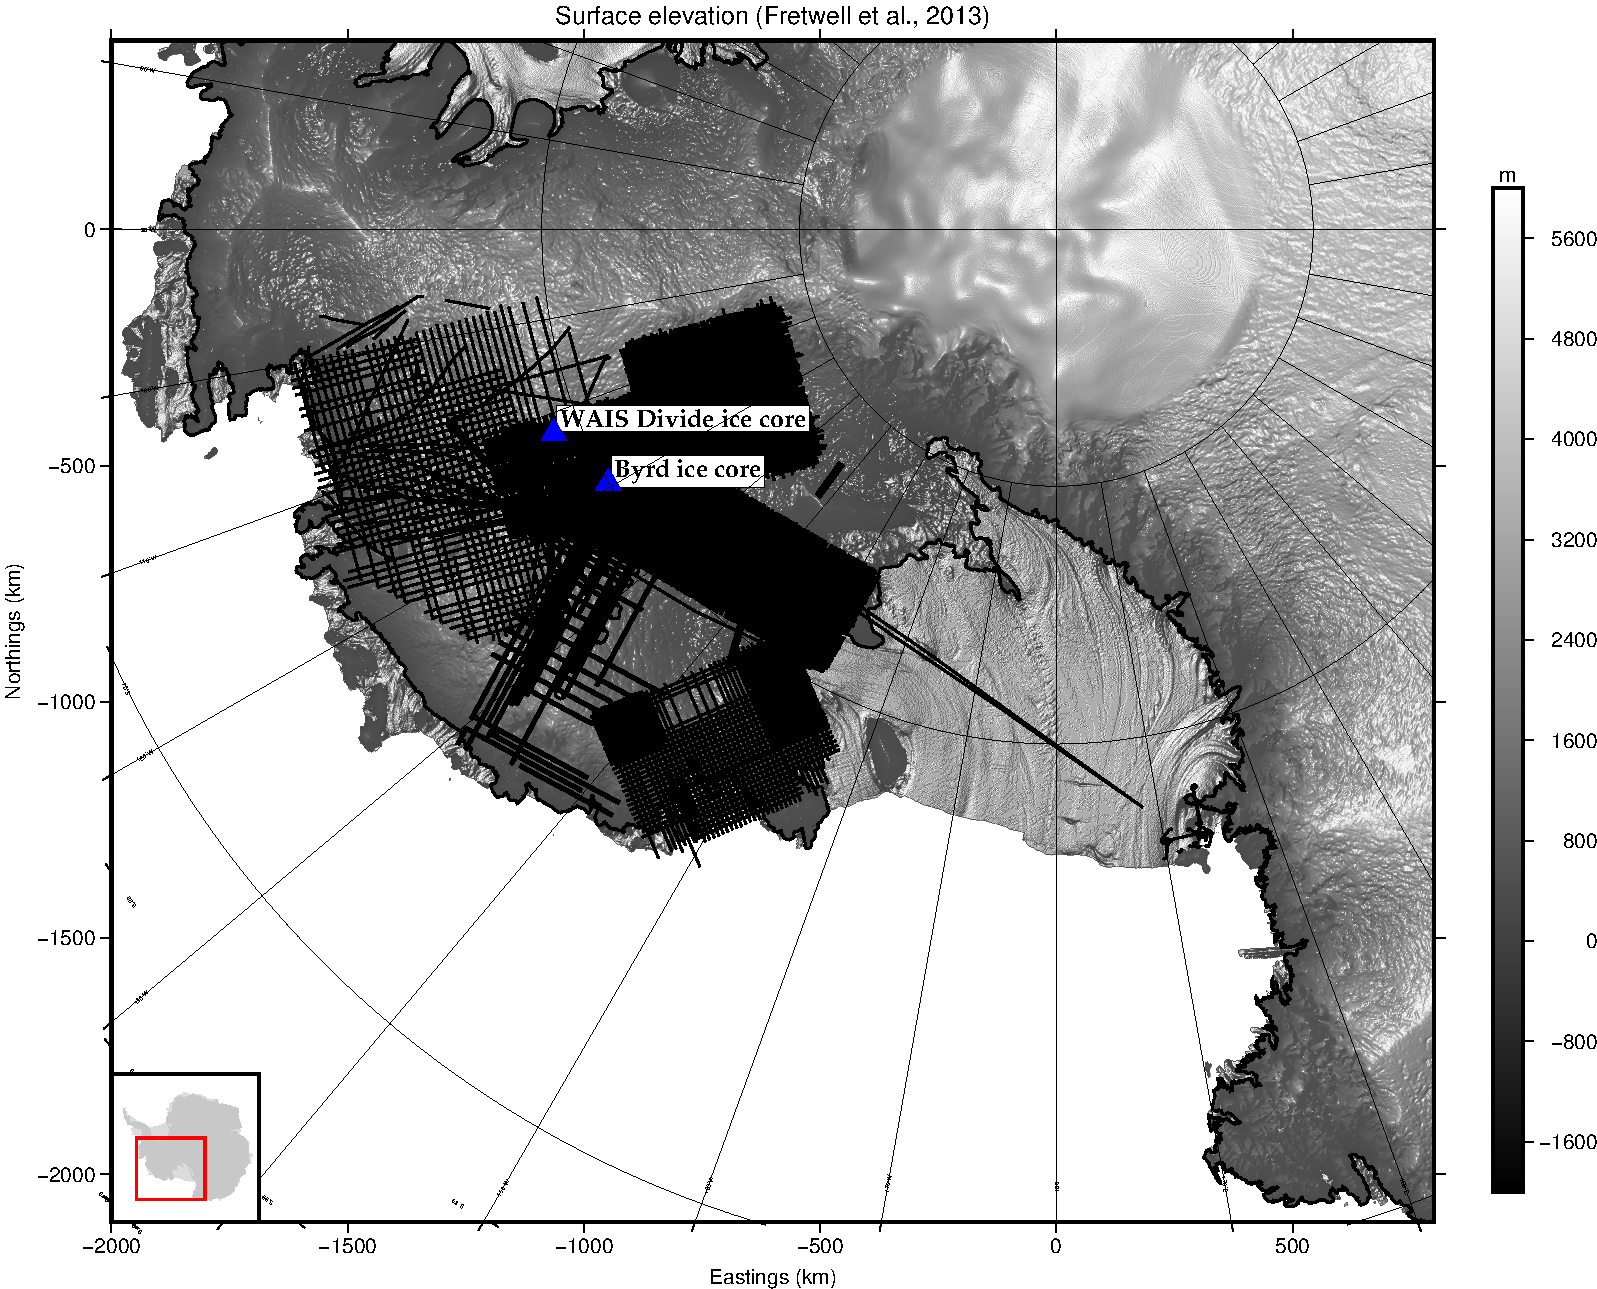
\includegraphics[scale=0.6]{figures/WAISall_dem_flat_pst_cores}
%\captionsetup{width=.9\textwidth}
\caption[]{Map of central West Antarctic with available airborne geophysical radar surveys (black lines) and WAIS Divide and Byrd ice core locations (blue triangles) overlain. Gray shading is surface elevation according to Fretwell et al. 2013. }
%\end{center}
\label{fig:radarmap}
\end{figure}


\begin{figure}[!htbp]
%\begin{center}
\centering
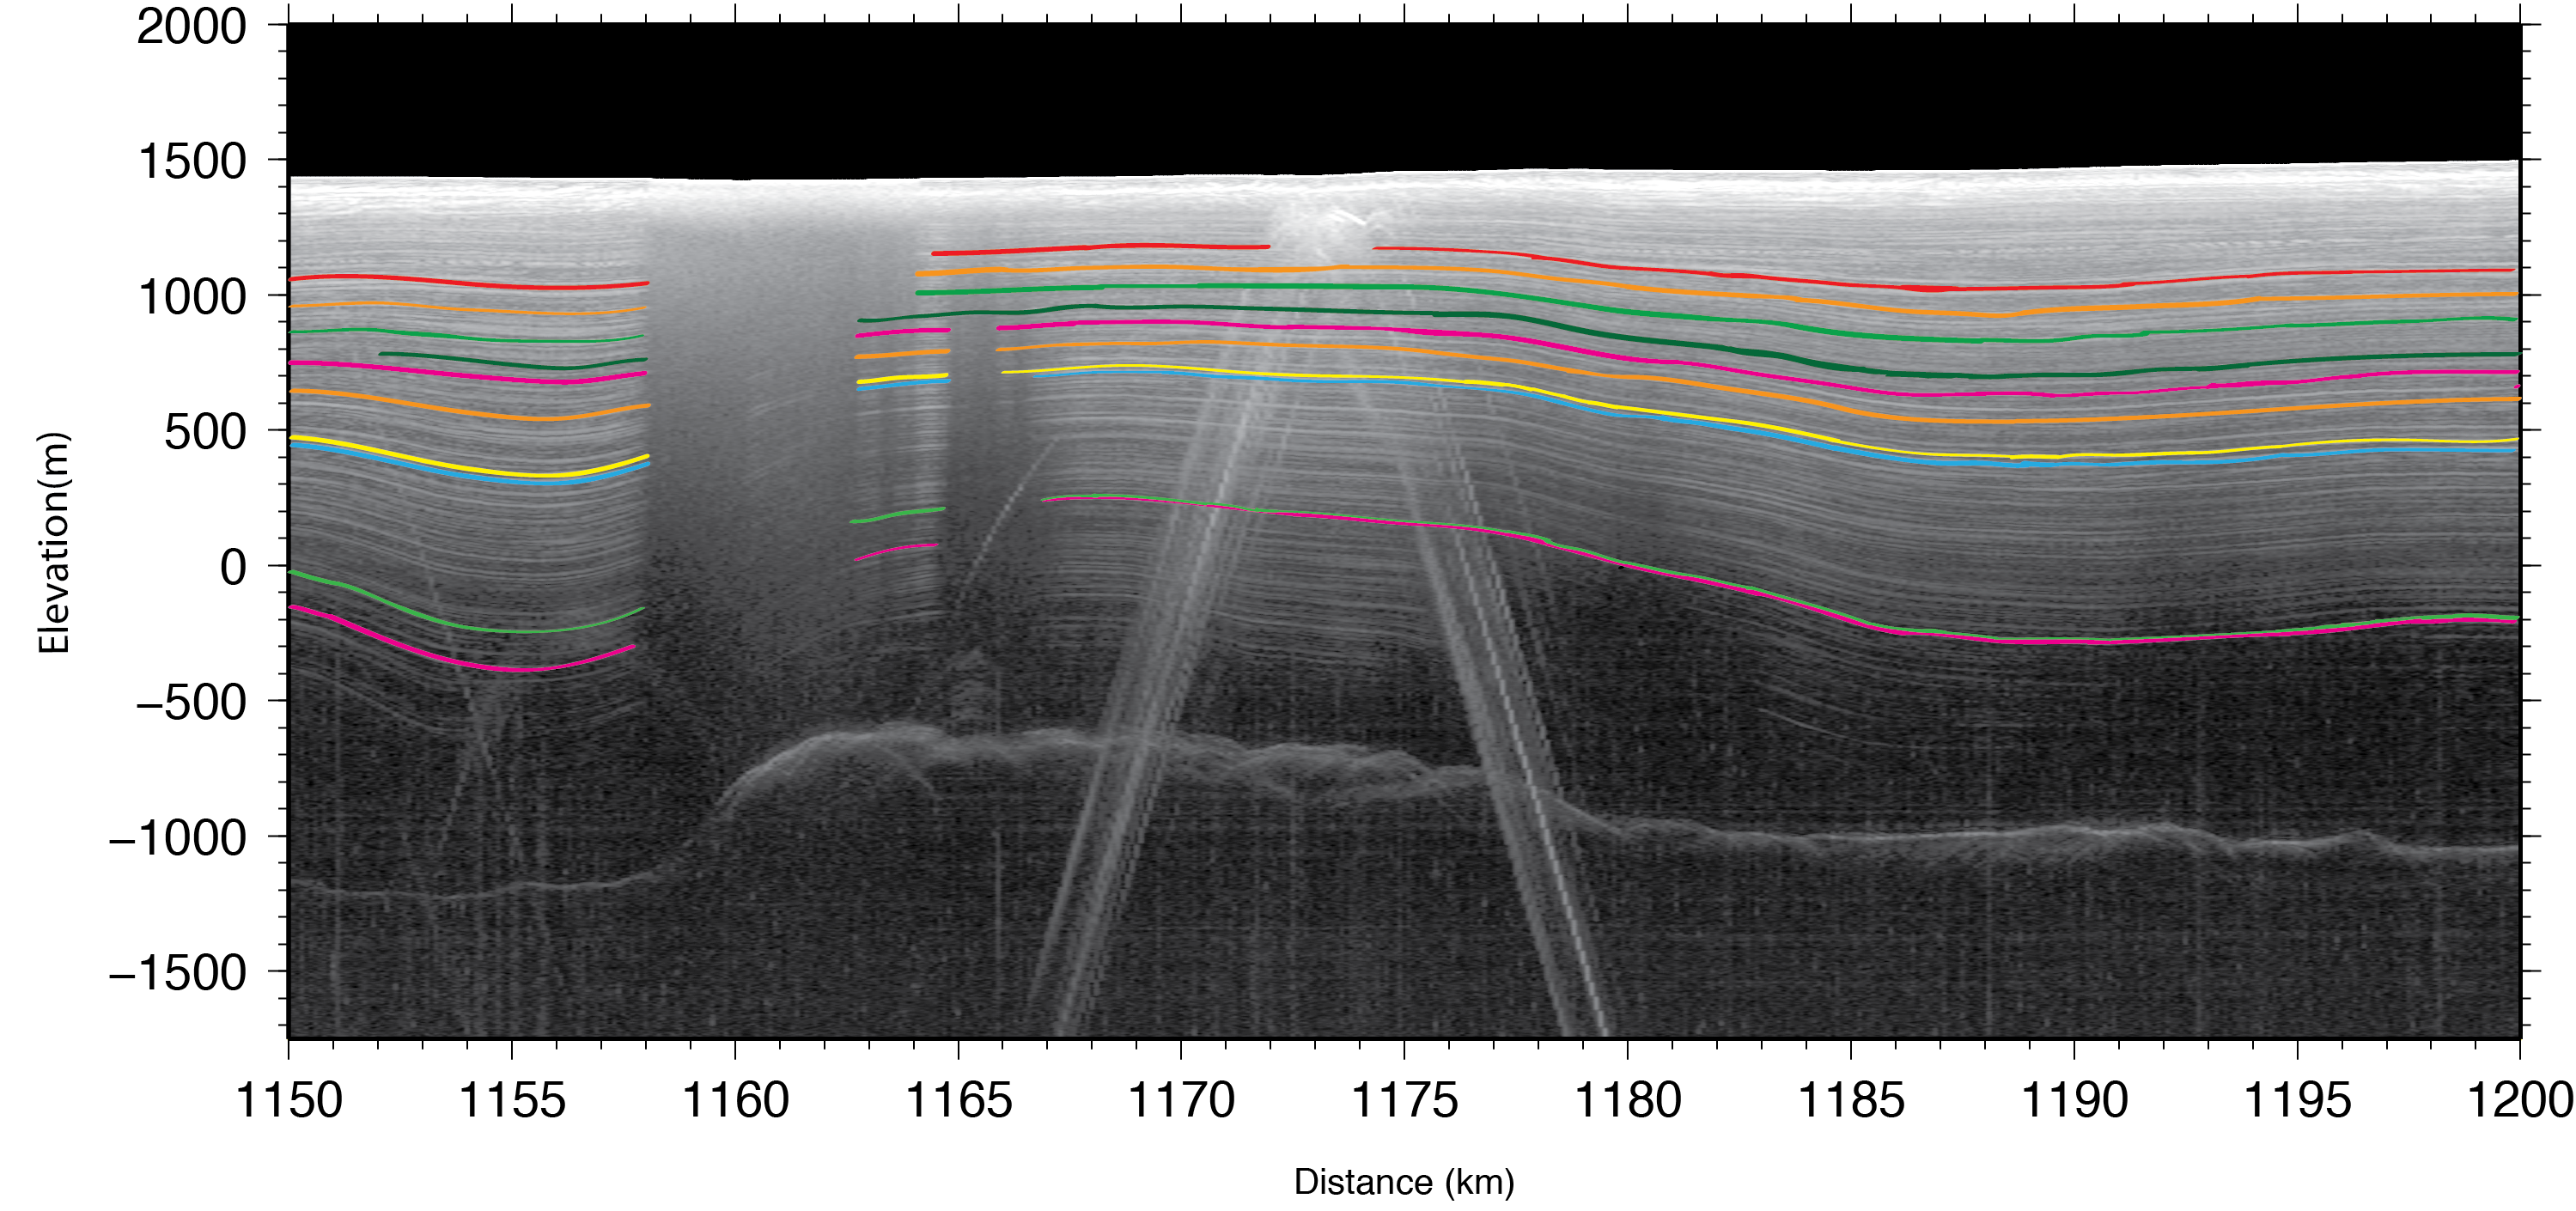
\includegraphics[scale=0.55]{figures/radargram}
%\captionsetup{width=.9\textwidth}
\caption[]{\textbf{a)} Spatial extent of 10 englacial horizons tracked through the WAIS for this study. \textbf{b)} Radargram of the area observed near Byrd ice core highlighting the ten radar horizons analyzed. The arrow on top of the figure indicates the location of the horizontal position of radar observations used. Our analysis shows that Horizons 7 and 8 and Horizons 9 and 10 are consistent within uncertainty to belonging to the same isochrone, though they appear distinct in the radargram. This emphasizes the importance of uncertainty quantification in interpretation of these horizons. }
%\end{center}
\label{fig:radargram}
\end{figure}


\begin{figure}[ht]
\begin{center}
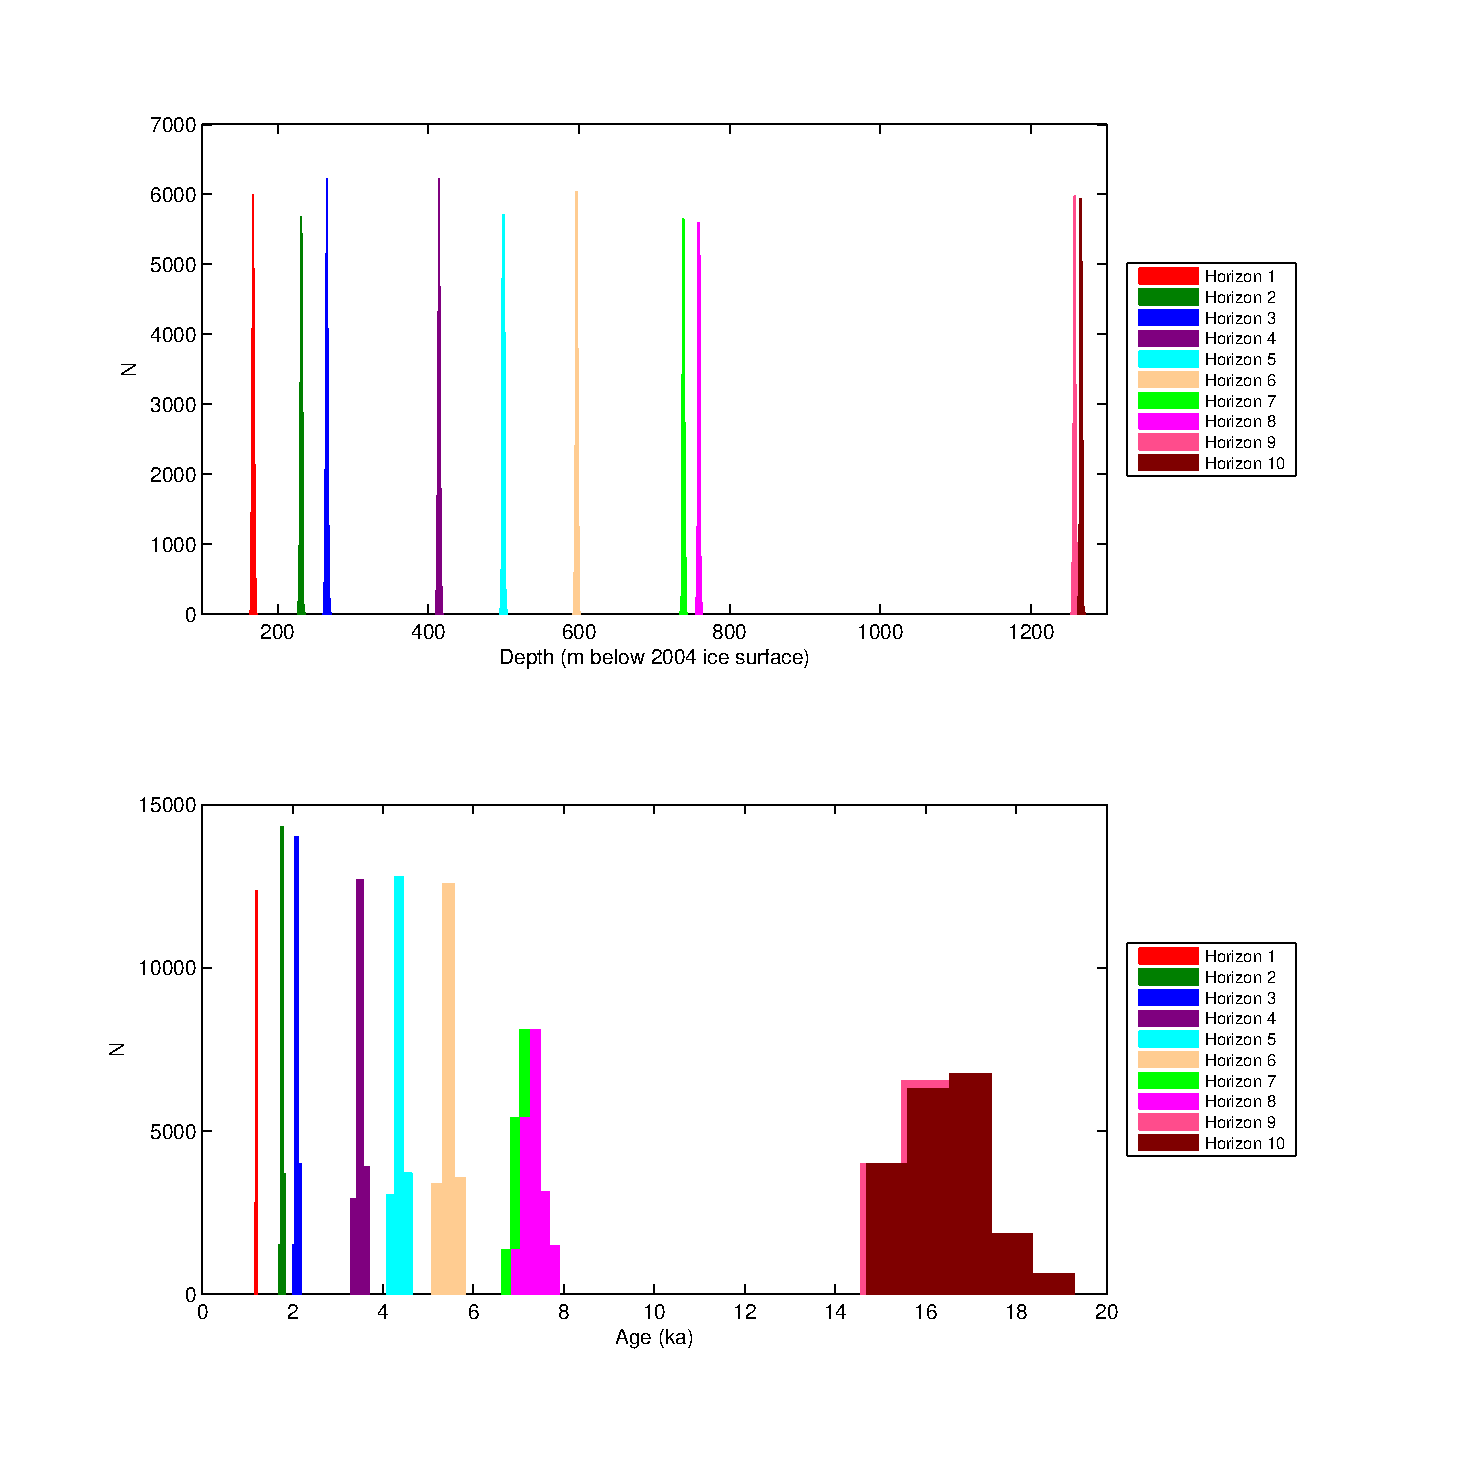
\includegraphics[scale=0.59]{figures/agedepthhist_morland}
\captionsetup{width=.9\textwidth}
\caption{a) Histogram of modeled water-equivalent ice depth for each of ten prominent radar horizons observed using airborne radar near Byrd Station, West Antarctica. The width of each distribution is the result of uncertainties arising from the method of radar collection. b) Similar histogram in terms of age (ka). Age uncertainty comes from approximate uncertainty in ice core dating techniques. }
\label{fig:agedepthhist}
\end{center}
\end{figure}


\begin{figure}[ht]
\begin{center}
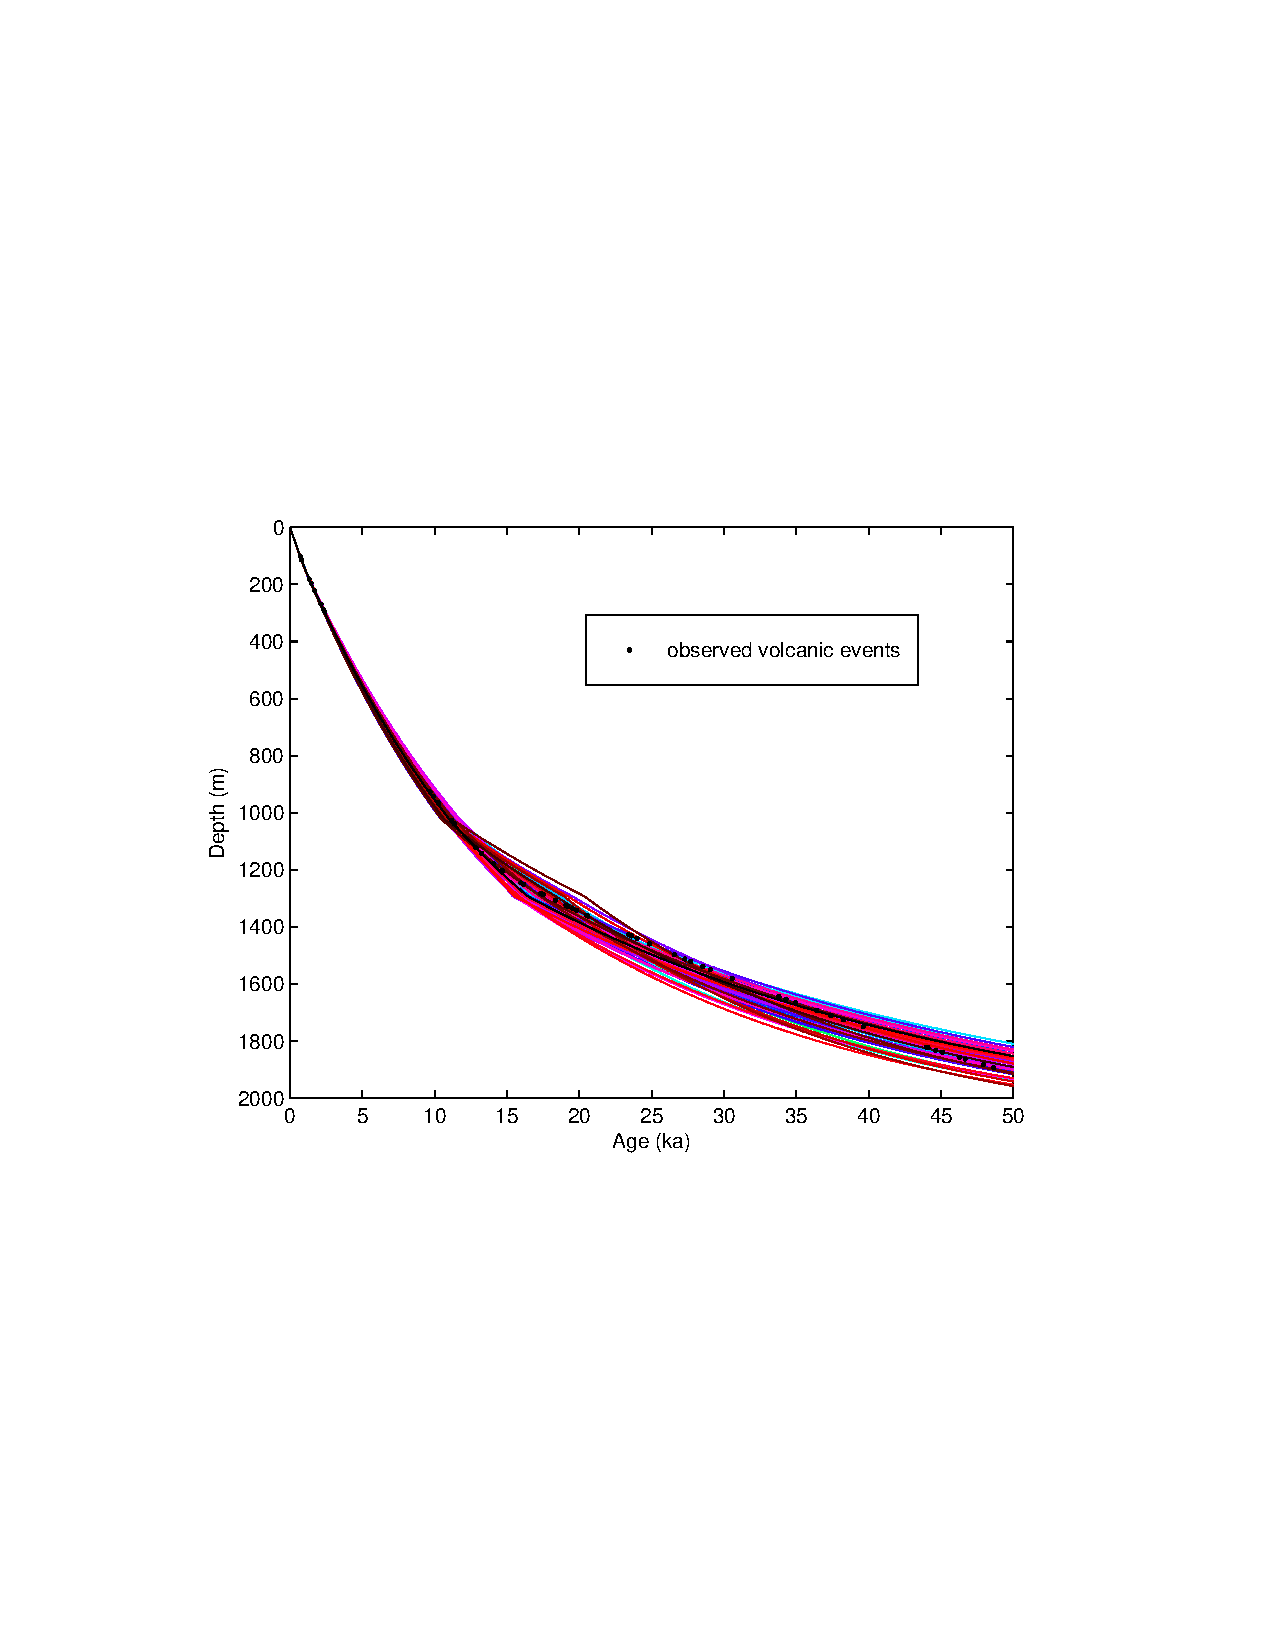
\includegraphics[scale=0.75]{figures/agedepth_metrop}
\captionsetup{width=.9\textwidth}
\vspace*{-10mm}
\caption{ Ensemble of modeled age-depth profiles near Byrd ice core.  Black dots represent dated volcanic events from the Byrd ice core record \citep{hammer1994}. Each line represents a set of parameters that describe the observed data within uncertainty. (See Section~$\ref{method}$.)   }
\label{fig:spaghetti}
\end{center}
\end{figure}

\begin{figure}[ht]
\begin{center}
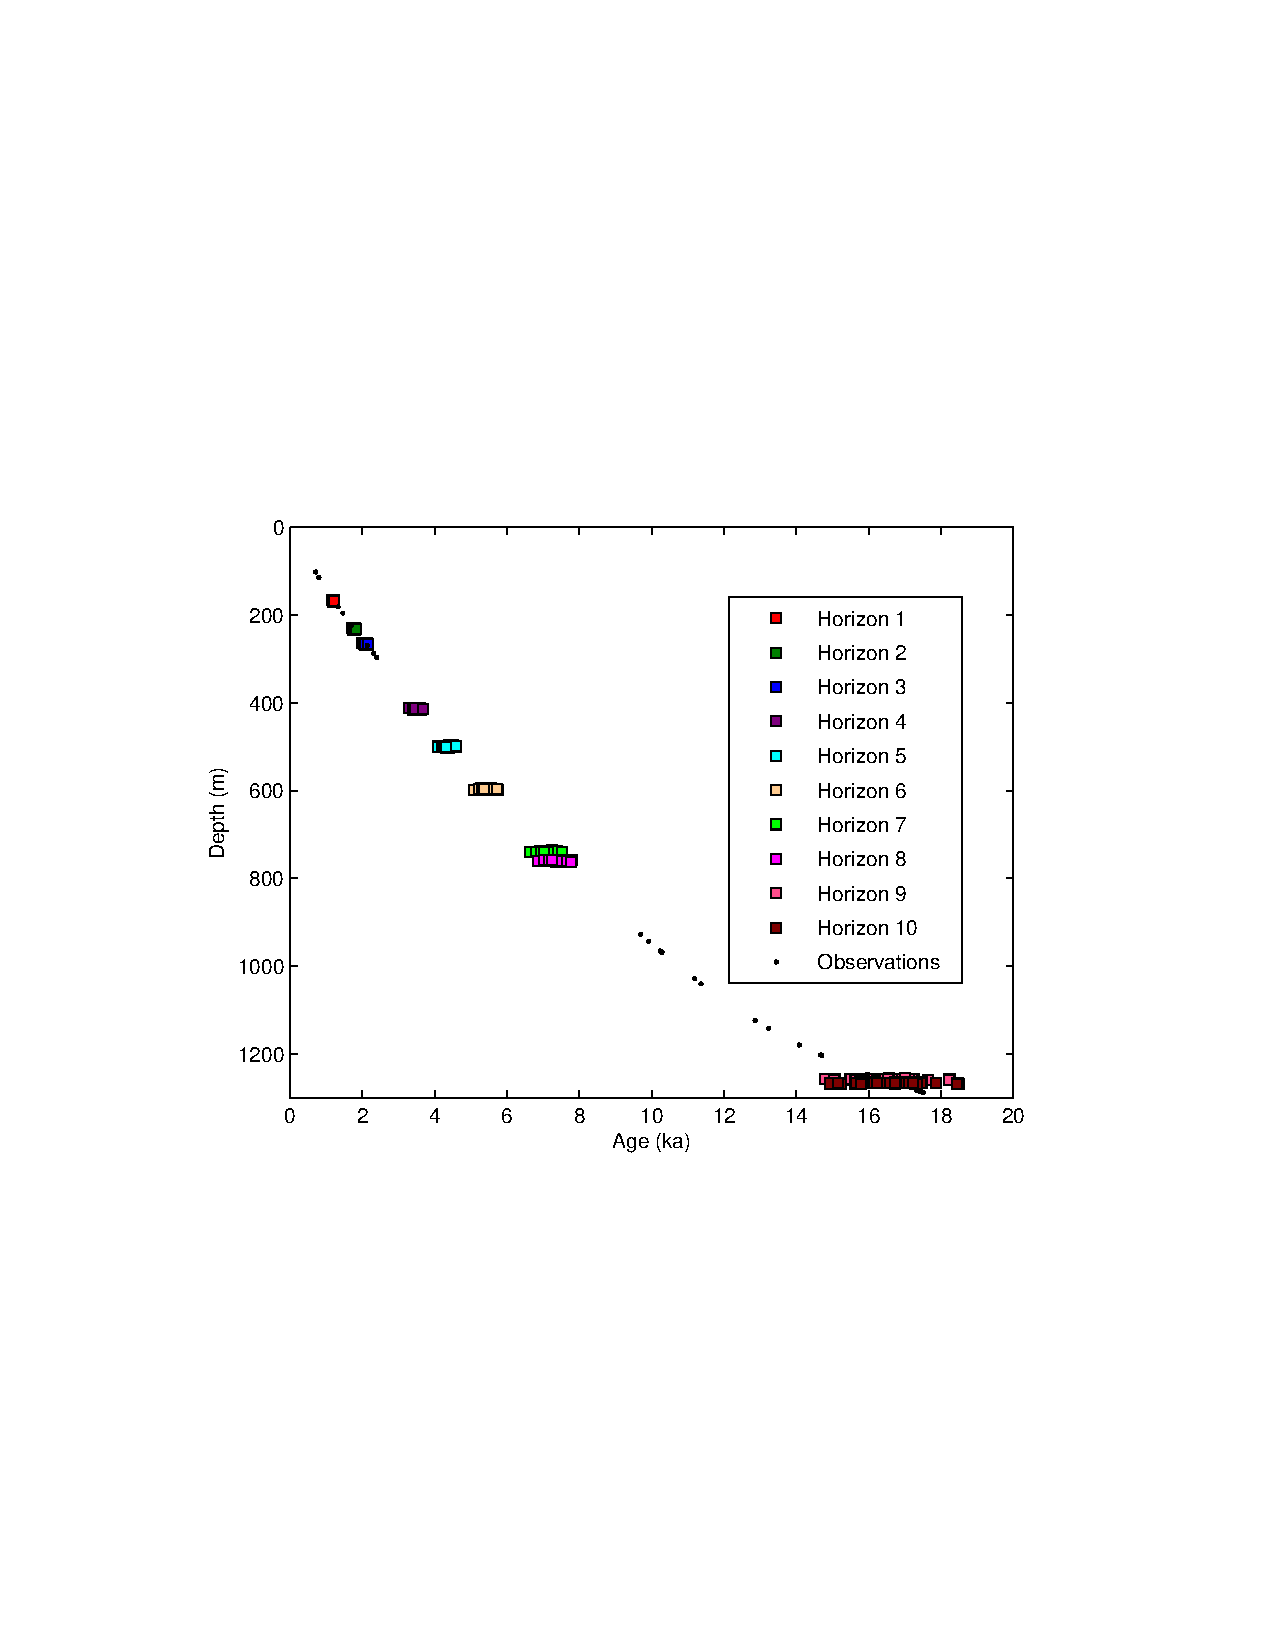
\includegraphics[scale=0.75]{figures/hor_agedepth_morland}
\captionsetup{width=.9\textwidth}
\caption{ Age-depth profile of ten prominent radar horizons compared to an observed volcanic age-depth profile of the Byrd ice core. The depth and age of each radar horizon are randomly sampled within uncertainty to obtain an ensemble of possible values for that horizon.  }
\label{fig:horagedepth}
\end{center}
\end{figure}


\begin{figure}[ht]
\begin{center}
%\begin{array}{cc}
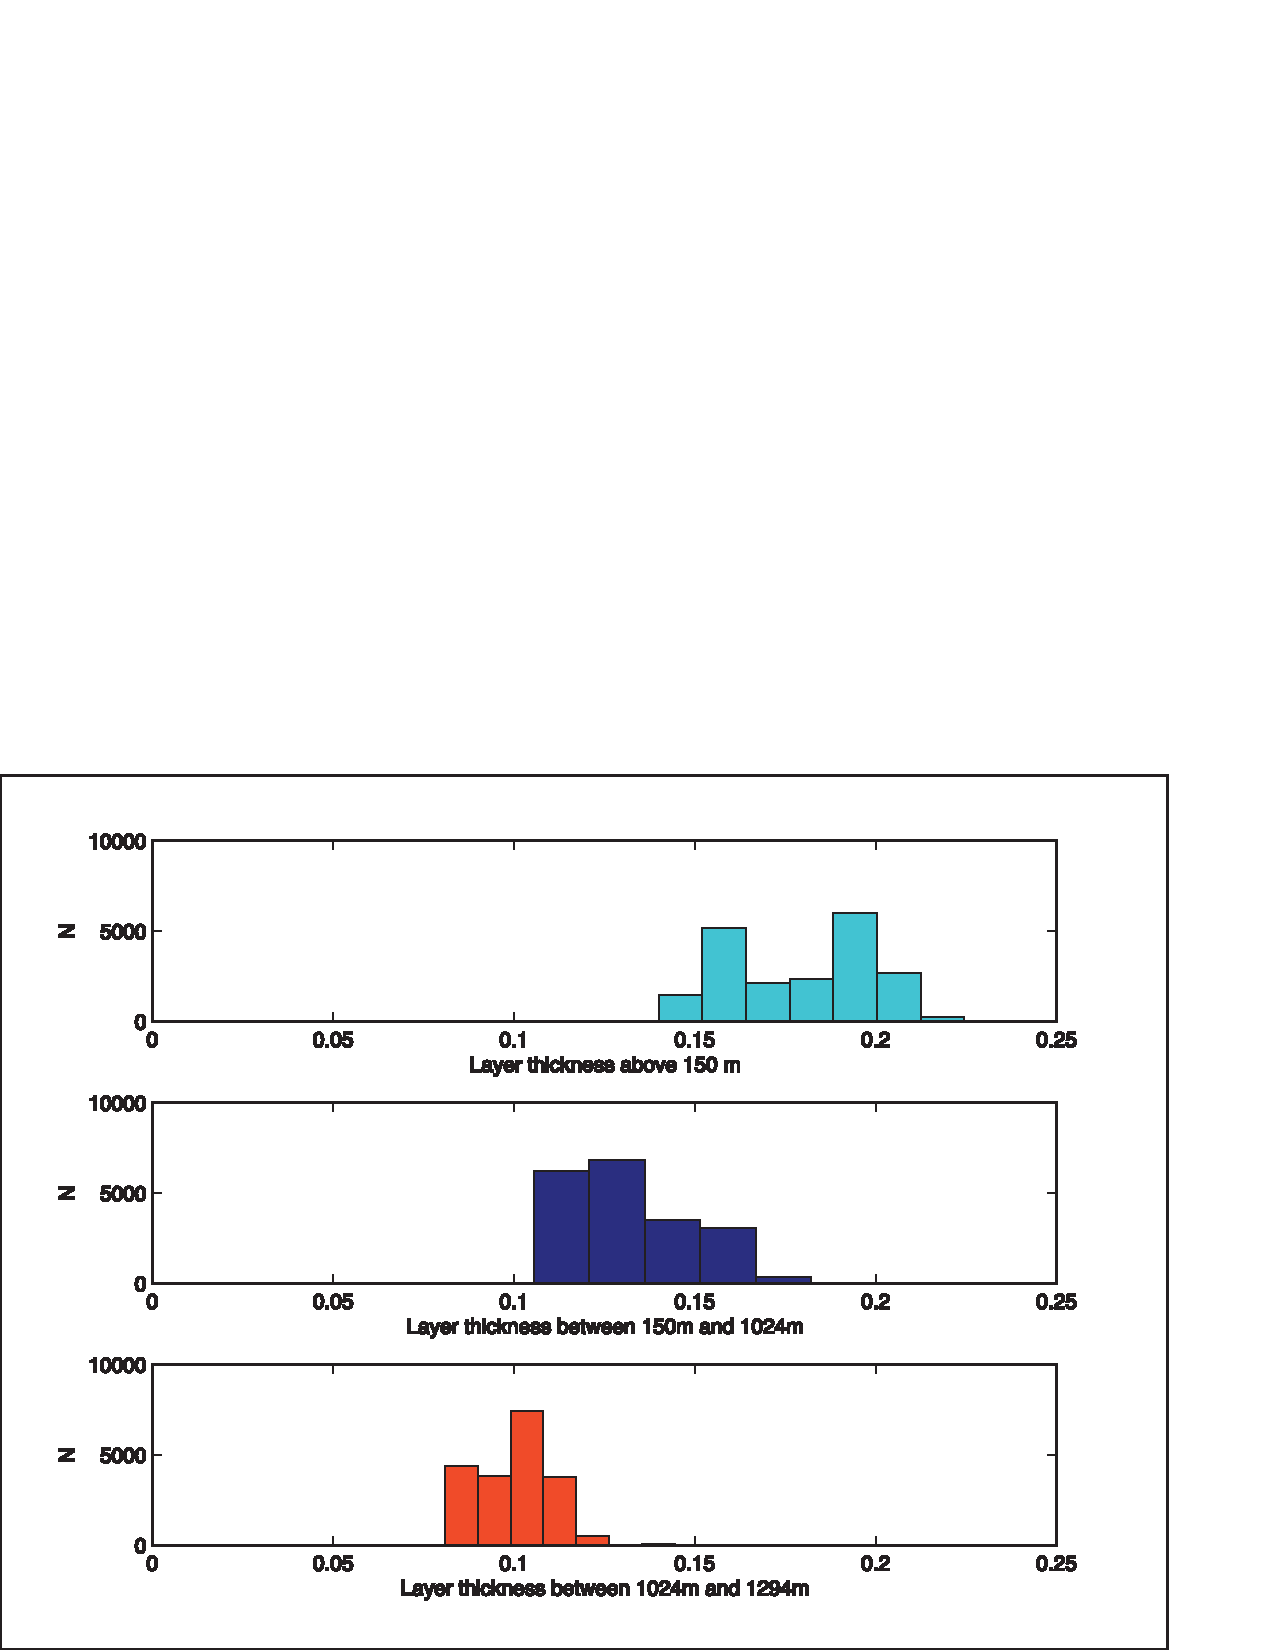
\includegraphics[scale=0.75]{figures/layerthk_v3_10ksamples}
%\end{array}$
%\end{center}
%\captionsetup{width=.9\textwidth}
\caption{Modeled layer thickness in each of four depth regimes near Byrd Station, West Antarctica. The model overestimates layer thickness, particularly in deeper regimes. }
\label{fig:accum}
\end{center}
\end{figure}


\begin{table}[ht]
\centering
\begin{tabular}{|c|c|c|}
\hline
Depth Range (m) & \multicolumn{1}{c|}{Layer thickness} & \multicolumn{1}{c|}{Median Layer thickness}  \\
& at Divide (m) & at Byrd  (m)\\
\hline
$\textit{d}$ $<$ 150 & $\sim$ 0.27 &  0.16 $\pm$ 0.04\\
150 $<$ $\textit{d}$ $<$ 1024 & $\sim$ 0.14 - 0.27 & 0.13  $\pm$ 0.06\\
1024 $<$ $\textit{d}$ $<$ 1294 & $\sim$ 0.08 - 0.14 & 0.10 $\pm$ 0.04\\
%$\textit{d}$ $>$ 1294 $<$ &  $\sim$ 0.08 -  0.20 & 0.19 $\pm$ 0.05\\
\hline
\end{tabular}
\captionsetup{width=.9\textwidth}
\caption{Comparison between layer thickness at the Western Divide between the Ross and Amundson Seas \citep{neumann2008} and modeled here at Byrd Station. Maximum layer thickness occurs at the divide, so layer thicknesses at Byrd Station are expected to be less, but comparable, at Byrd Station. We find that layer thickness at Byrd is the same as layer thickness at the Divide to within uncertainty, implying that our model is overestimating layer thickness. This is especially the case at depth, where we expect layer thinning to decrease the thickness of deeper layers due to increased strain. Uncertainties shown are at the 2$\sigma$ level.}
\label{table:accums}
\end{table}

%\begin{table}\label{age_unc}
%\begin{tabular}{|p{4cm}|p{4cm}|p{8cm}|}
%\hline
% Age (a) & 1$\sigma$ Uncertainty (a) & Method of Dating  \\
%\hline
%&&\\
%Age $<$ 1360 & $\pm$ 2  & ECM method on a shallow follow-up ice core, NBY89 from \citep{langway1994}\\
%& & \\
%1360 $\ge$ Age $>$ 11500 & $\pm$ 150  & end of Younger Dryas period and $^{10}Be$ peak ]\citep{blunier1998} \\
%&& \\
%11500 $\ge$ Age $>$ 17320 & $\pm$ 300 & significant volcanic event "Old Faithful" from \citet{hammer1994}\\
%&&\\
%Age $\ge$ 17320 & $\pm$ 2000 & U/Th dating of Laschamp geomagnatic excursion \citep{schramm2000}\\
%\hline
%\end{tabular}
%\captionsetup{width=.9\textwidth}
%\caption{Uncertainty in Byrd ice core chronology Age uncertainty is considered to be gaussian with standard deviation from a variety of age reference points.}
%\tablenotetext{a}{Footnote text here.}
%\end{table}


\vspace*{-10mm}
\begin{table}[ht]
\centering
\begin{tabular}{| c | c || c | c | c || c | c | c |}
\hline
\multirow{2}{*}{Horizon} & \multicolumn{1}{c||}{TWTT} &  \multicolumn{3}{c||}{Depth (m)} & \multicolumn{3}{c|}{Age (a)} \\   
\cline{3-8}
& ($\mu$s)& Mean & Median & $\sigma$ & Mean & Median & $\sigma$ \\
\hline
 1 & 6.02   & 167.6  & 167.6  & 2.4 & 1200 & 1200 & 20   \\
 2 & 6.78   & 231.4  & 231.4  & 2.4 & 1770 & 1770 & 40   \\
 3 & 7.18   & 265.6  & 265.6  & 2.3 & 2100 & 2100 & 60  \\
 4 & 8.94   & 414.4  & 414.4  & 2.4 & 3510 & 3500 & 150   \\
 5 & 9.94   & 499.6  & 499.6  & 2.4 & 4360 & 4360 & 200   \\
 6 & 11.10  & 596.9  & 596.9  & 2.3 & 5440 & 5440 & 270   \\
 7 & 12.78  & 738.8  & 738.8  & 2.3 & 7120 & 7110 & 370   \\
 8 & 13.02  & 759.1  & 759.1  & 2.3 & 7350 & 7340 & 390   \\
 9 & 18.92  & 1257.7 & 1257.7 & 2.4 & 16220 & 16300 & 1760   \\
 10& 19.02  & 1266.2 & 1266.2 & 2.3 & 16400 & 16500 & 1820  \\
\hline
\end{tabular}
%\tablenotetext{a}{Footnote text here.}
\captionsetup{width=.9\textwidth}
\caption{Depth and age mean, median, and uncertainty for ten strong radar reflectors near Byrd Station, West Antarctica. The radar two-way travel time (TWTT) is given in column 1. }
\end{table}
\label{table:results}
\end{document}

